\documentclass[a4paper,14pt]{extarticle}

\usepackage[utf8x]{inputenc}
\usepackage[T1,T2A]{fontenc}
\usepackage[russian]{babel}
\usepackage{hyperref}
\usepackage{indentfirst}
\usepackage{here}
\usepackage{array}
\usepackage{graphicx}
\usepackage{caption}
\usepackage{subcaption}
\usepackage{chngcntr}
\usepackage{amsmath}
\usepackage{amssymb}
\usepackage{pgfplots}
\usepackage{pgfplotstable}
\usepackage[left=2cm,right=2cm,top=2cm,bottom=2cm,bindingoffset=0cm]{geometry}
\usepackage{multicol}

\renewcommand{\le}{\ensuremath{\leqslant}}
\renewcommand{\leq}{\ensuremath{\leqslant}}
\renewcommand{\ge}{\ensuremath{\geqslant}}
\renewcommand{\geq}{\ensuremath{\geqslant}}
\renewcommand{\epsilon}{\ensuremath{\varepsilon}}
\renewcommand{\phi}{\ensuremath{\varphi}}

\counterwithin{figure}{section}
\counterwithin{equation}{section}
\counterwithin{table}{section}
\newcommand{\sign}[1][5cm]{\makebox[#1]{\hrulefill}} % Поля подписи и даты
\graphicspath{{pics/}} % Путь до папки с картинками
\captionsetup{justification=centering,margin=1cm}
\def\arraystretch{1.3}

\usepackage{courier}

\usepackage{listings}
\lstset{ %
extendedchars=\true,
keepspaces=true,
language=C,						% choose the language of the code
basicstyle=\footnotesize,		% the size of the fonts that are used for the code
numbers=left,					% where to put the line-numbers
numberstyle=\footnotesize,		% the size of the fonts that are used for the line-numbers
stepnumber=1,					% the step between two line-numbers. If it is 1 each line will be numbered
numbersep=5pt,					% how far the line-numbers are from the code
backgroundcolor=\color{white},	% choose the background color. You must add \usepackage{color}
showspaces=false				% show spaces adding particular underscores
showstringspaces=false,			% underline spaces within strings
showtabs=false,					% show tabs within strings adding particular underscores
frame=single,           		% adds a frame around the code
tabsize=2,						% sets default tabsize to 2 spaces
captionpos=b,					% sets the caption-position to bottom
breaklines=true,				% sets automatic line breaking
breakatwhitespace=false,		% sets if automatic breaks should only happen at whitespace
escapeinside={\%*}{*)},			% if you want to add a comment within your code
postbreak=\raisebox{0ex}[0ex][0ex]{\ensuremath{\color{red}\hookrightarrow\space}},
texcl=true,
}

\lstset{basicstyle=\footnotesize\ttfamily,breaklines=true}

\begin{document}

\begin{titlepage}
\begin{center}
	\textbf{Санкт-Петербургский Политехнический Университет \\Петра Великого}\\[0.3cm]
	\small Институт компьютерных наук и технологий \\[0.3cm]
	\small Кафедра компьютерных систем и программных технологий\\[4cm]
	
	\textbf{ОТЧЕТ}\\ \textbf{о лабораторной работе}\\[0.5cm]
	\textbf{<<Использование стандартных подпрограмм для приближенного\\ вычисления интеграла>>}\\[0.1cm]
	\textbf{Вычислительная математика}\\[8.0cm]
\end{center}

\begin{flushright}
	\begin{minipage}{0.48\textwidth}
		\begin{flushleft}
			\small \textbf{Работу выполнил студент}\\[3mm]
			\small группа 23501/4 \hspace*{6mm} Дьячков В.В.\\[5mm]
			
			\small \textbf{Преподаватель}\\[5mm]
		 	\small \sign[3cm] \hspace*{5mm} к.т.н., доц. Цыган В.Н.\\[0.5cm]
		\end{flushleft}
	\end{minipage}
\end{flushright}

\vfill

\begin{center}
	\small Санкт-Петербург\\
	\small \the\year
\end{center}
\end{titlepage}

\section{Техническое задание}

\textbf{Задание К-3-08:} Дана консольная балка с переменным поперечным сечением, показанная на рисунке \ref{img:balka}.

\begin{figure}[H]
\begin{center}
	\vspace{-0.5cm}
	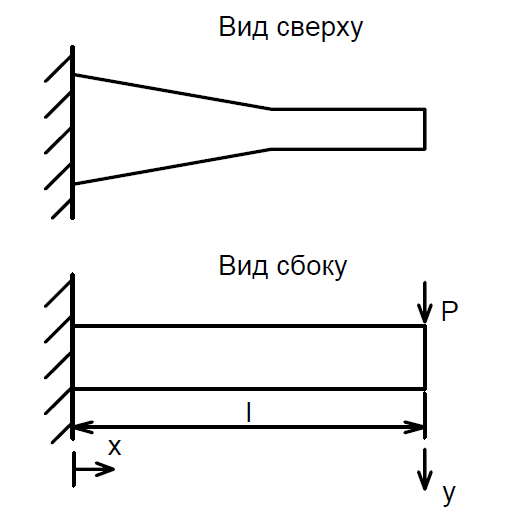
\includegraphics[scale=0.45]{balka}
	\caption{Консольная балка}
	\label{img:balka}
	\vspace{-0.5cm}
\end{center}
\end{figure}

Дифференциальное уравнение для вертикального прогиба имеет вид:
\[
\frac{d^4y}{dx^4} = - \frac{2}{I} \frac{dI}{dx}\cdot \frac{d^3y}{dx^3} -  \frac{1}{I} \frac{d^2I}{dx^2}\cdot \frac{d^2y}{dx^2} + \frac{\omega}{EI},
\]
где $x$ -- горизонтальное расстояние вдоль балки, $y$ -- вертикальный прогиб, $l$ -- длина балки, $M$ -- изгибающий момент, $E$ -- модуль Юнга, $I$ -- момент инерции, $P$ -- нагрузка на балку.

\begin{center}
\begin{multicols}{2}
$\omega = - \frac{d^2M}{dx^2}$

$M(x) = -P \cdot (l - x)$
\end{multicols}
\end{center}

\begin{center}
\begin{multicols}{2}
$E = 3\cdot 10^7$

$I(x) = 5 \cdot (1 + 4 e^{-\frac{6x}{l}})$
\end{multicols}
\end{center}

Начальные условия:
\begin{center}
\begin{multicols}{3}
$y(0) = y'(0) = 0$

$y''(0) = \frac{Pl}{75}\cdot 10^{-7}$

$y'''(0) = \frac{P \cdot 3.8}{75}\cdot 10^{-7}$
\end{multicols}
\end{center}

Вычислить $y(l)$ для различных значений $P$. Построить сплайн по значениям $y(l)$ в зависимости от $P$ и с его помощью оценить $y(l)$ для $P_0$. 

Оценить погрешность результата и влияние на точность погрешности исходных данных.

\section{Исходные данные}

Значения нагрузки на балку: $500 \le P \le 1000$ с шагом $100$, $P_0 = 750$.

Значения длины балки: $l = 50\cdot x^*$, где $x^*$ -- корень уравнения \ref{eq:int} на промежутке $[1, 4]$.

\begin{equation}\label{eq:int}
\int_0^{20} \frac{e^{-0.9z}}{z+x}dz = 0.1957981\cdot x
\end{equation}

\section{Выполнение работы}

\section{Результаты}

\section*{Приложение}

\captionof{lstlisting}{main.h}
\lstinputlisting[
	basicstyle=\scriptsize,	
	numberstyle=\scriptsize,
	label=code:mainh
]{main.h}

\captionof{lstlisting}{main.cpp}
\lstinputlisting[
	basicstyle=\scriptsize,	
	numberstyle=\scriptsize,
	label=code:maincpp
]{main.cpp}

\end{document}